% Options for packages loaded elsewhere
\PassOptionsToPackage{unicode}{hyperref}
\PassOptionsToPackage{hyphens}{url}
%
\documentclass[
]{article}
\usepackage{amsmath,amssymb}
\usepackage{lmodern}
\usepackage{iftex}
\ifPDFTeX
  \usepackage[T1]{fontenc}
  \usepackage[utf8]{inputenc}
  \usepackage{textcomp} % provide euro and other symbols
\else % if luatex or xetex
  \usepackage{unicode-math}
  \defaultfontfeatures{Scale=MatchLowercase}
  \defaultfontfeatures[\rmfamily]{Ligatures=TeX,Scale=1}
\fi
% Use upquote if available, for straight quotes in verbatim environments
\IfFileExists{upquote.sty}{\usepackage{upquote}}{}
\IfFileExists{microtype.sty}{% use microtype if available
  \usepackage[]{microtype}
  \UseMicrotypeSet[protrusion]{basicmath} % disable protrusion for tt fonts
}{}
\makeatletter
\@ifundefined{KOMAClassName}{% if non-KOMA class
  \IfFileExists{parskip.sty}{%
    \usepackage{parskip}
  }{% else
    \setlength{\parindent}{0pt}
    \setlength{\parskip}{6pt plus 2pt minus 1pt}}
}{% if KOMA class
  \KOMAoptions{parskip=half}}
\makeatother
\usepackage{xcolor}
\usepackage[margin=1in]{geometry}
\usepackage{longtable,booktabs,array}
\usepackage{calc} % for calculating minipage widths
% Correct order of tables after \paragraph or \subparagraph
\usepackage{etoolbox}
\makeatletter
\patchcmd\longtable{\par}{\if@noskipsec\mbox{}\fi\par}{}{}
\makeatother
% Allow footnotes in longtable head/foot
\IfFileExists{footnotehyper.sty}{\usepackage{footnotehyper}}{\usepackage{footnote}}
\makesavenoteenv{longtable}
\usepackage{graphicx}
\makeatletter
\def\maxwidth{\ifdim\Gin@nat@width>\linewidth\linewidth\else\Gin@nat@width\fi}
\def\maxheight{\ifdim\Gin@nat@height>\textheight\textheight\else\Gin@nat@height\fi}
\makeatother
% Scale images if necessary, so that they will not overflow the page
% margins by default, and it is still possible to overwrite the defaults
% using explicit options in \includegraphics[width, height, ...]{}
\setkeys{Gin}{width=\maxwidth,height=\maxheight,keepaspectratio}
% Set default figure placement to htbp
\makeatletter
\def\fps@figure{htbp}
\makeatother
\setlength{\emergencystretch}{3em} % prevent overfull lines
\providecommand{\tightlist}{%
  \setlength{\itemsep}{0pt}\setlength{\parskip}{0pt}}
\setcounter{secnumdepth}{5}
\newlength{\cslhangindent}
\setlength{\cslhangindent}{1.5em}
\newlength{\csllabelwidth}
\setlength{\csllabelwidth}{3em}
\newlength{\cslentryspacingunit} % times entry-spacing
\setlength{\cslentryspacingunit}{\parskip}
\newenvironment{CSLReferences}[2] % #1 hanging-ident, #2 entry spacing
 {% don't indent paragraphs
  \setlength{\parindent}{0pt}
  % turn on hanging indent if param 1 is 1
  \ifodd #1
  \let\oldpar\par
  \def\par{\hangindent=\cslhangindent\oldpar}
  \fi
  % set entry spacing
  \setlength{\parskip}{#2\cslentryspacingunit}
 }%
 {}
\usepackage{calc}
\newcommand{\CSLBlock}[1]{#1\hfill\break}
\newcommand{\CSLLeftMargin}[1]{\parbox[t]{\csllabelwidth}{#1}}
\newcommand{\CSLRightInline}[1]{\parbox[t]{\linewidth - \csllabelwidth}{#1}\break}
\newcommand{\CSLIndent}[1]{\hspace{\cslhangindent}#1}
\ifLuaTeX
  \usepackage{selnolig}  % disable illegal ligatures
\fi
\IfFileExists{bookmark.sty}{\usepackage{bookmark}}{\usepackage{hyperref}}
\IfFileExists{xurl.sty}{\usepackage{xurl}}{} % add URL line breaks if available
\urlstyle{same} % disable monospaced font for URLs
\hypersetup{
  hidelinks,
  pdfcreator={LaTeX via pandoc}}

\title{Neural correlates of the uncanny valley effect\\
for robots and hyper-realistic masks\\
(for submission to Computers in Human Behavior)}
\author{Shona Fitzpatrick, Ailish K. Byrne, Alex Headley, Jet G. Sanders,\\
Helen Petrie, Rob Jenkins \& Daniel H. Baker}
\date{2023-01-02}

\begin{document}
\maketitle

\hypertarget{abstract}{%
\section{Abstract}\label{abstract}}

\hypertarget{introduction}{%
\section{Introduction}\label{introduction}}

Many people report an aversion to entities that are human-like, but on closer inspection are actually artificial. Examples include humanoid robots (androids), puppets, realistic computer-generated images, and hyper-realistic masks. The term `uncanny valley' (Mori, 1970; English translation in Mori et al., 2012) describes the idea that entities that are clearly human or clearly artificial do not evoke unease, whereas artificial entities that are human-like are disconcerting. Understanding these experiences is increasingly important as artificial entities become more integrated into our everyday lives, however at present relatively little is known about the neural underpinnings of the uncanny valley effect.

Neural responses to faces and bodies in general are well-characterised, and there appear to be specialised brain regions devoted to both (reviewed in Hu et al., 2020). For example, areas of the occipital lobe (Gauthier et al., 2000) and fusiform gyrus (Kanwisher et al., 1997) respond more to faces than non-face stimuli, and sections of extrastriate cortex are responsive to bodies (Downing et al., 2001). There are also event-related potential (ERP) signals associated with face and body stimuli, though their precise purpose is still debated (Thierry et al., 2007). It seems highly likely that `uncanny' images will activate these same processes, yet it is unclear whether the sense of unease they produce occurs at bottom-up sensory stages, or is modulated by more top-down cognitive factors.

One previous study has measured fMRI responses to moving stimuli designed to elicit an uncanny valley effect. Saygin et al. (2012) found repetition suppression effects in action-specific brain regions responding to movies of androids that had a biological appearance, but mechanical motion. These effects were stronger than for movies of humans or mechanical robots performing the same actions. A more recent electroencephalography (EEG) study (Urgen et al., 2018) identified a difference in the N400 component between dynamic and static conditions using the same stimuli. Although this difference was strongest over frontal electrodes, source reconstruction of the N400 itself suggested a left-lateralised source in temporo-parietal cortex, consistent with the fMRI results (Saygin et al., 2012). The authors interpret both of these findings as being due to the discrepancy between the human-like appearance and the clearly non-biological motion of the robot.

Our aim here was to further investigate neural correlates of the uncanny valley effect. We achieve this through two EEG experiments, in which we measure neural responses to static images. In the first experiment, the stimuli were humans, machine-like robots, and human-like robots. In the second experiment we aimed to generalise the finding by using images of people wearing no masks, wearing obvious masks (e.g.~carnival or halloween masks), and wearing hyper-realistic silicone masks (Sanders et al., 2017). Rather than focus on specific ERP components, we use a non-parametric cluster correction procedure to compare conditions. We also apply a pattern classification approach to identify time windows in which information in the EEG signal can be used to distinguish between pairs of conditions.

\hypertarget{materials-methods}{%
\section{Materials \& Methods}\label{materials-methods}}

\hypertarget{participants}{%
\subsection{Participants}\label{participants}}

A total of 29 participants completed Experiment 1 (12 male, 17 female), and 30 participants completed Experiment 2 (7 male, 23 female). None of the participants had previously taken part in a study using these stimuli, and all were naïve to the hypotheses and wore their normal optical correction if required. Written informed consent was collected before each experiment began, and all procedures were approved by the Ethics committee of the Department of Psychology at the University of York.

\hypertarget{apparatus-stimuli}{%
\subsection{Apparatus \& stimuli}\label{apparatus-stimuli}}

In Experiment 1, the stimulus set consisted of a total of 90 images, evenly split between three categories: real faces, human-like robots, and mechanical robots. Images all showed the head and shoulders of the subject, had white backgrounds, and were sourced from the internet. In Experiment 2, the stimulus set consisted of a total of 296 images, comprising real faces (148 images), people wearing silicone masks (74 images), and people wearing Halloween masks (74 images). The backgrounds of these images were more heterogeneous, and showed the natural surroundings of the subject. In both experiments, images involved examples of both genders, and of varied ethnic backgrounds.

All stimuli were displayed on a ViewPixx display running at 120Hz, controlled by an Apple Macintosh computer. The display was gamma corrected using a photometer to ensure that the luminance output was linear. EEG data were collected using a 64-channel Waveguard cap and an ANT Neuroscan system, sampling at 1kHz. Low latency digital triggers were sent between the display and the EEG amplifier using an 8-bit parallel cable.

\hypertarget{procedure}{%
\subsection{Procedure}\label{procedure}}

\hypertarget{experiment-1-robots}{%
\subsubsection{Experiment 1: robots}\label{experiment-1-robots}}

Each participant completed three blocks of the first experiment. Within each block, all 90 stimulus images were presented twice in a random order. Stimuli subtended \(11\times11\) degrees at the viewing distance of 57cm, and were shown against a mid-grey background, with a black central fixation cross displayed throughout. The presentation duration was 500ms, and participants were asked to press a mouse button to indicate if they believed each image was of a human or of a robot. After each response there was a random duration blank period with a mean duration of 1000ms and a standard deviation of 200ms. Each block lasted around 6 minutes.

\hypertarget{experiment-2-hyper-realistic-masks}{%
\subsubsection{Experiment 2: hyper-realistic masks}\label{experiment-2-hyper-realistic-masks}}

Participants were shown all 296 images in a random order in each of three blocks. In the first block, stimuli subtended \(5.5\times7.5\) degrees of visual angle when viewed at a distance of 57cm. In the second block, stimuli doubled in size (width and height), and subtended \(11\times15\) degrees at the same viewing distance. In the third block, stimuli doubled in size again, and subtended \(22\times30\) degrees. Stimuli were presented for 250ms, and participants indicated whether they thought each image contained a real face or a mask, using a two-button trackball. The button assignment (whether the left button indicated a face or a mask, and vice versa) was determined randomly for each participant, but remained constant throughout the whole experiment. Text reminding the participant of the button assignment was present continuously in the lower right corner of the screen, far from the area of the screen where the stimuli were presented. A central fixation cross was also present throughout. After each response there was a random duration blank period with a mean duration of 1000ms and a standard deviation of 200ms. Each block lasted around 8 minutes.

\hypertarget{data-analysis}{%
\subsection{Data analysis}\label{data-analysis}}

EEG signals were recorded during each block, and saved to disc for subsequent offline analysis. We used a component of the EEGlab toolbox (Delorme and Makeig, 2004) to convert the continuous data from a proprietary file format to a compressed csv text file. All subsequent analyses were conducted in R using these files.

For each block, data at each electrode were low-pass filtered at 30Hz with a \(10^{th}\) order Butterworth filter, and then epoched using the stimulus onset triggers. A pre-stimulus baseline (average voltage of the 200ms before stimulus onset) was subtracted from each waveform. We rejected ERPs that showed evidence of excessive noise or movement artefacts on a per-electrode basis by excluding trials where the standard deviation across the time window from 200ms before to 1000ms after stimulus onset exceeded \(40\mu V\). ERPs were averaged across trials for each participant, and then across participants to calculate group averages.

We performed univariate analyses by conducting Bayesian t-tests (Rouder et al., 2009) between ERPs from pairs of conditions at each time point using a JZS prior. The resulting Bayes factor score is a summary of the evidence in favour of either the null hypothesis (that the waveforms are equal) or the alternative hypothesis (that they differ). We use the heuristics proposed by Jeffreys (1961) that Bayes factors \textgreater3 constitute some evidence supporting the alternative hypothesis, factors \textgreater10 constitute strong evidence, and factors \textgreater30 constitute very strong evidence.

Multivariate pattern analysis was conducted by training a linear support vector machine algorithm to discriminate between patterns of activity across electrodes at a specific time point. The patterns came from the real face condition and one of the mask conditions at a single stimulus size, and for a single participant. Examples of each pattern were calculated by averaging over random subsets of 36 trials from a given condition, and using these to train the classifier. The accuracy of the classifier was tested on the averaged remaining trials (that were not used in training) for each condition. This process was repeated 1000 times with different trial permutations to obtain an average accuracy, where chance performance is at 50\% correct. The analysis was carried out at all time points, and also for all participants. We then averaged classifier accuracy across participants, and calculated one sample Bayesian t-tests at each time point as described above.

\hypertarget{data-and-code-availability}{%
\subsection{Data and code availability}\label{data-and-code-availability}}

Raw data, processed data, and analysis scripts are freely available through the project repository at: \url{https://osf.io/5nz2h/}

\hypertarget{results}{%
\section{Results}\label{results}}

\hypertarget{experiment-1}{%
\subsection{Experiment 1}\label{experiment-1}}

\begin{figure}

{\centering 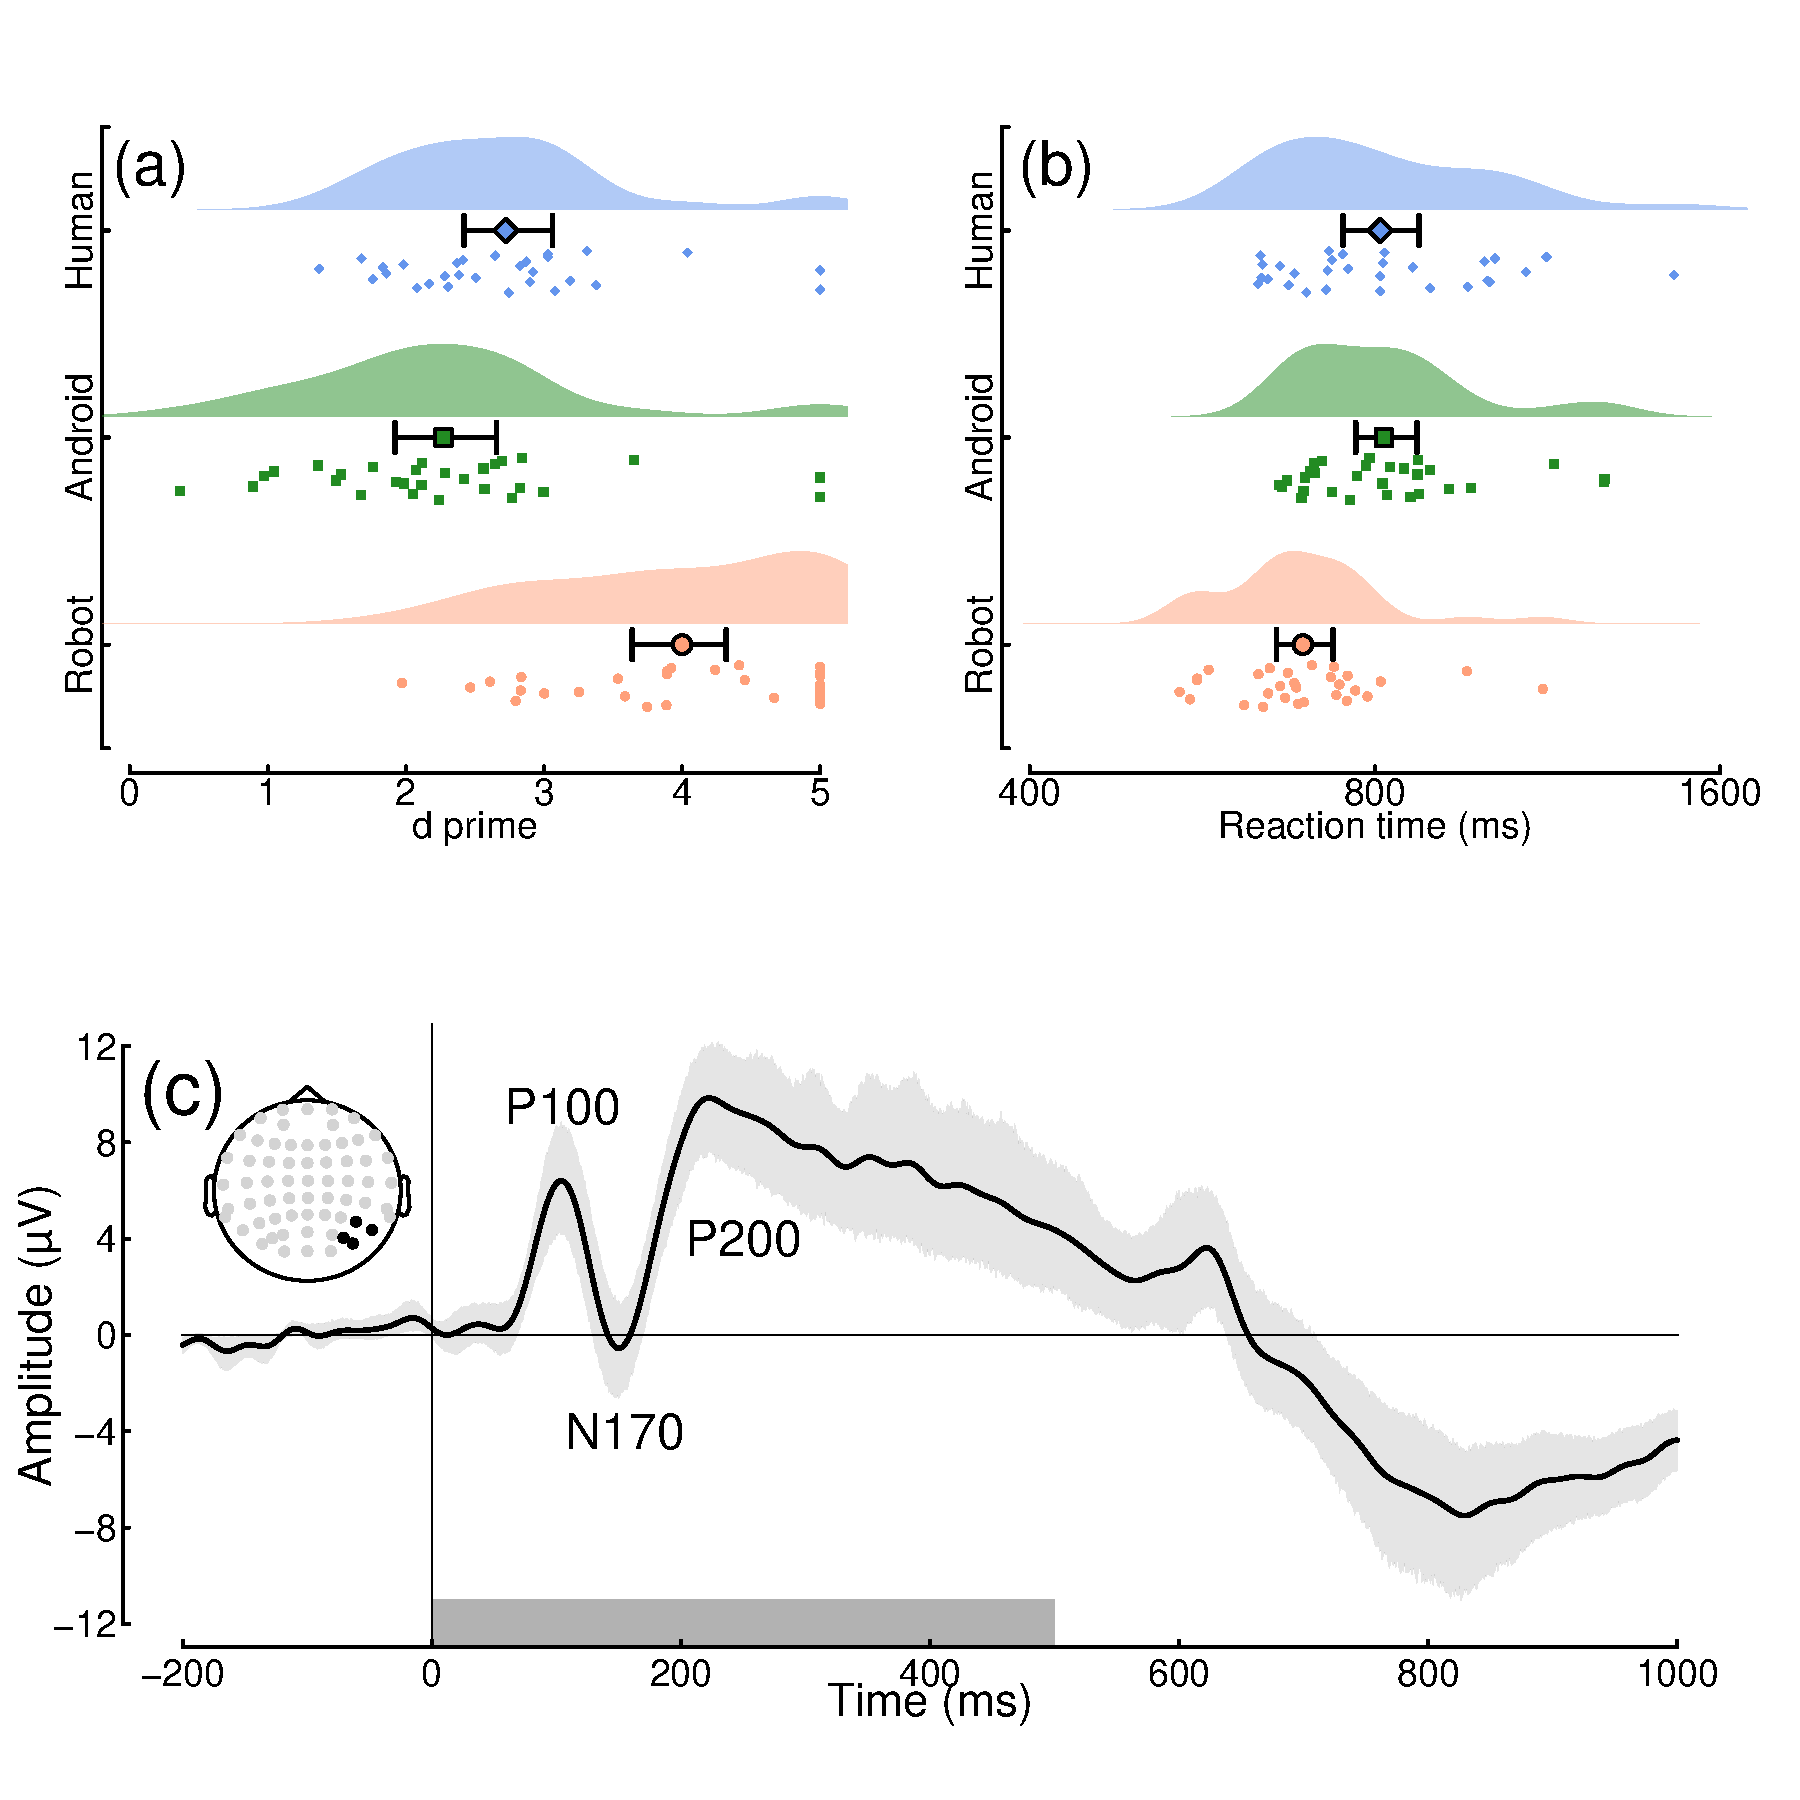
\includegraphics{Figures/RobotsData} 

}

\caption{I.}\label{fig:RobotsData}
\end{figure}

\begin{figure}

{\centering 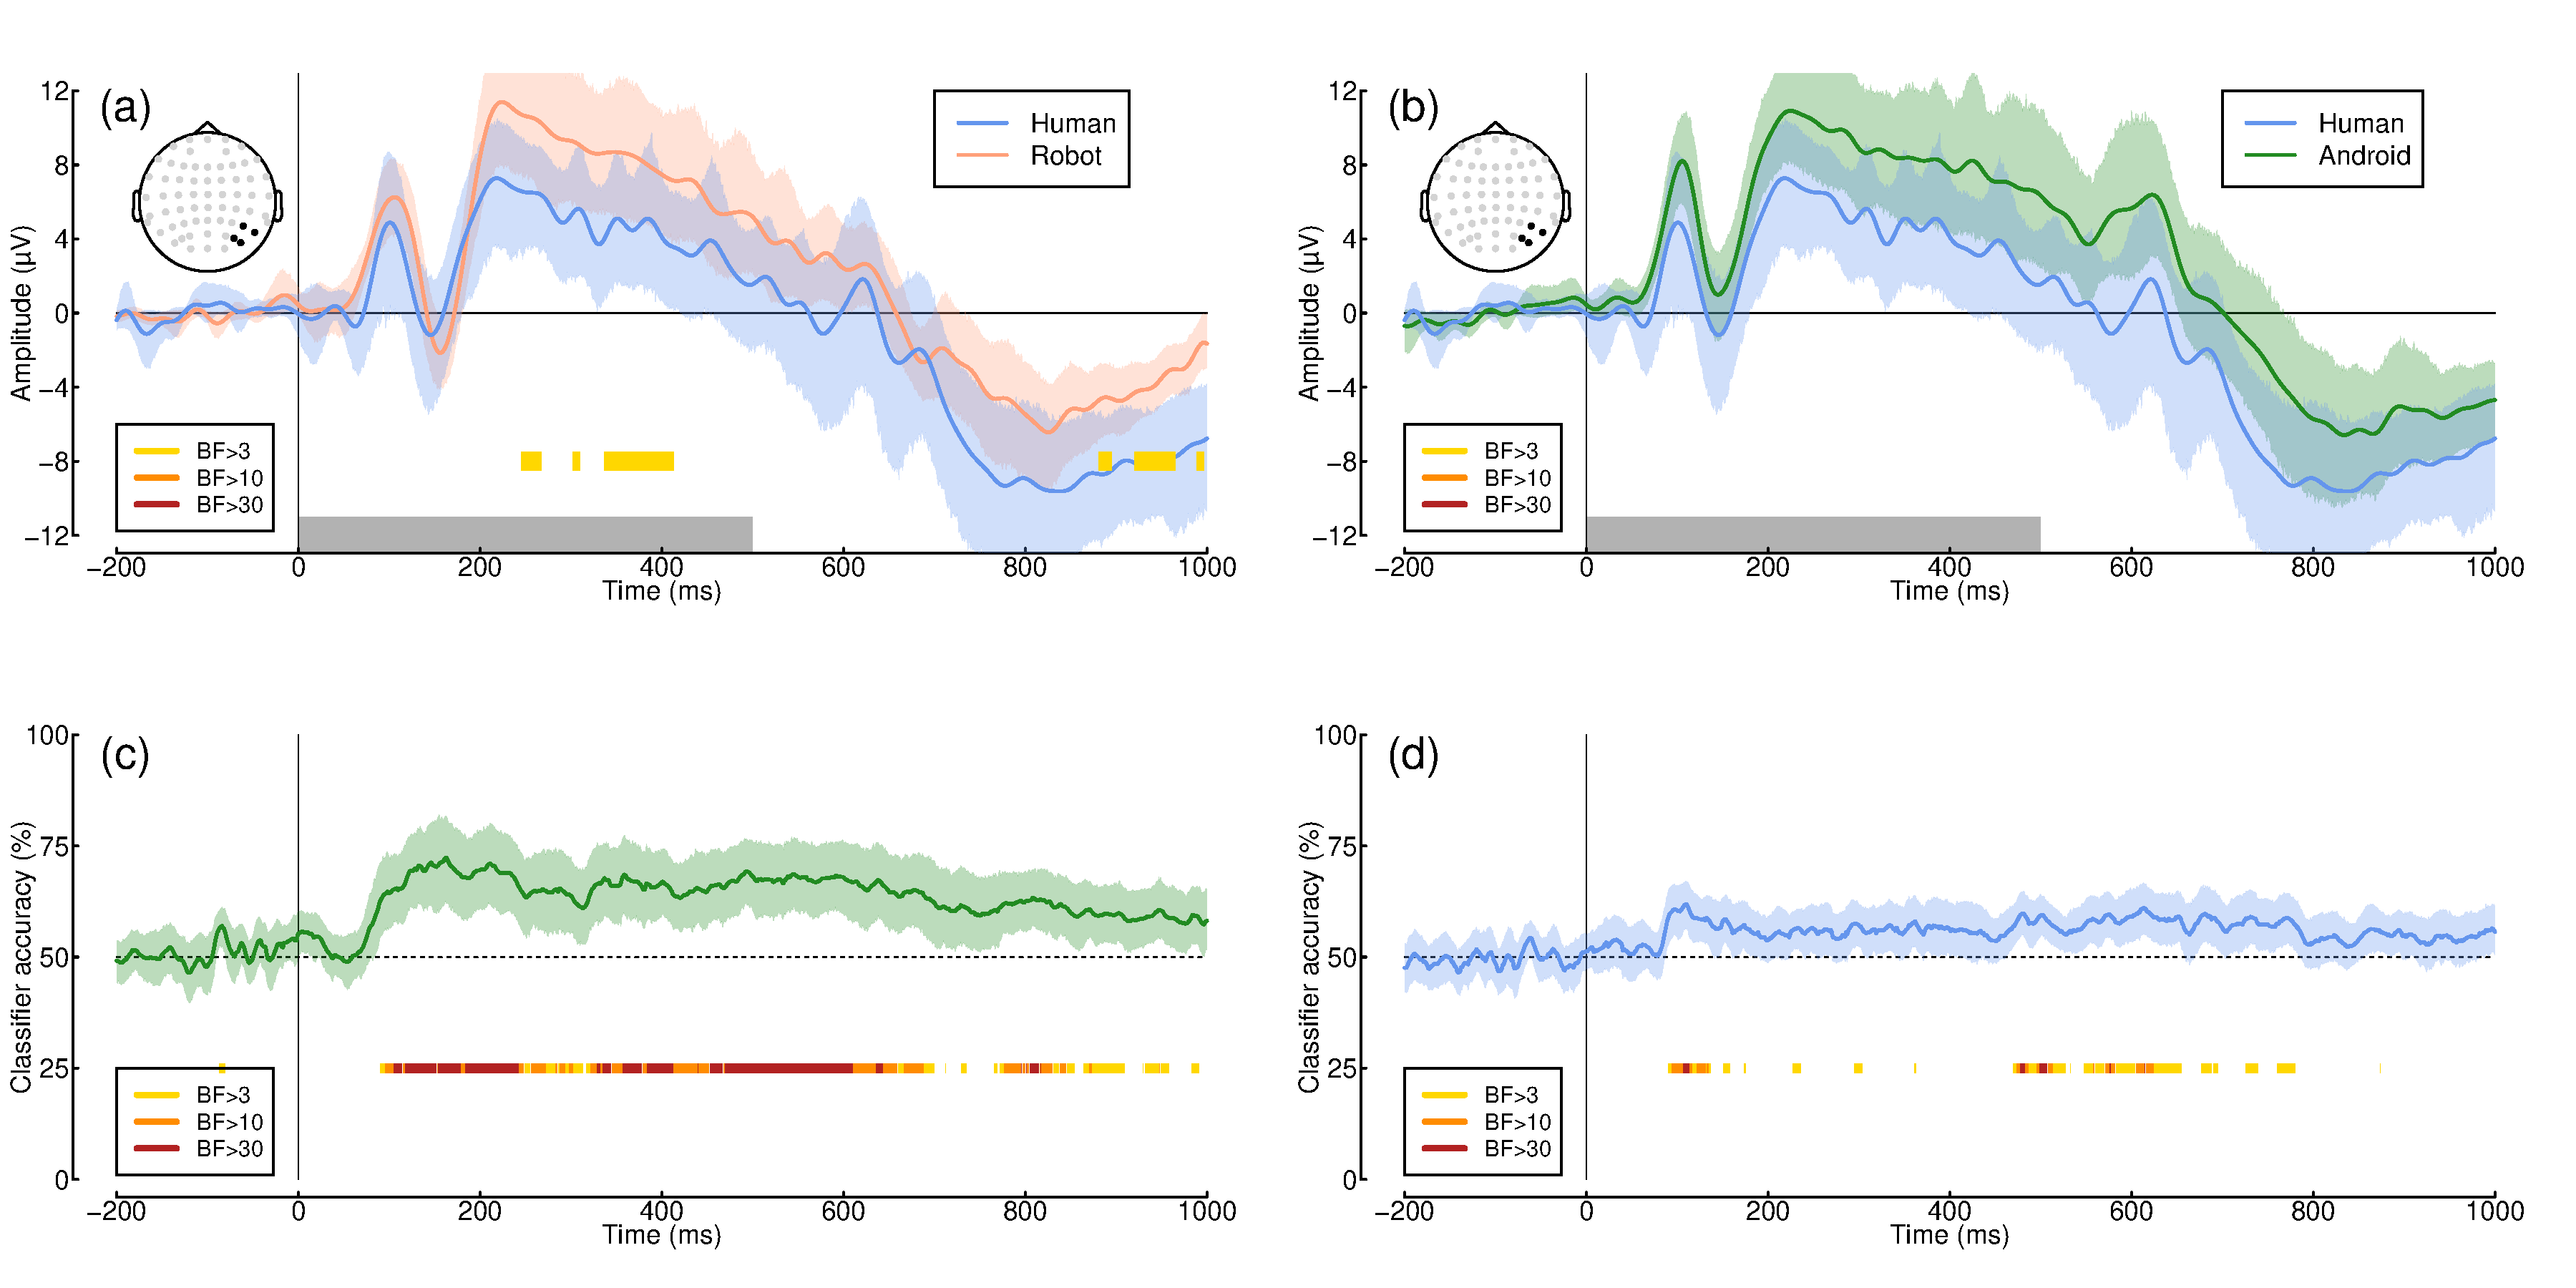
\includegraphics{Figures/RobotsMVPA} 

}

\caption{I.}\label{fig:RobotsMVPA}
\end{figure}

\hypertarget{experiment-2}{%
\subsection{Experiment 2}\label{experiment-2}}

\begin{figure}

{\centering 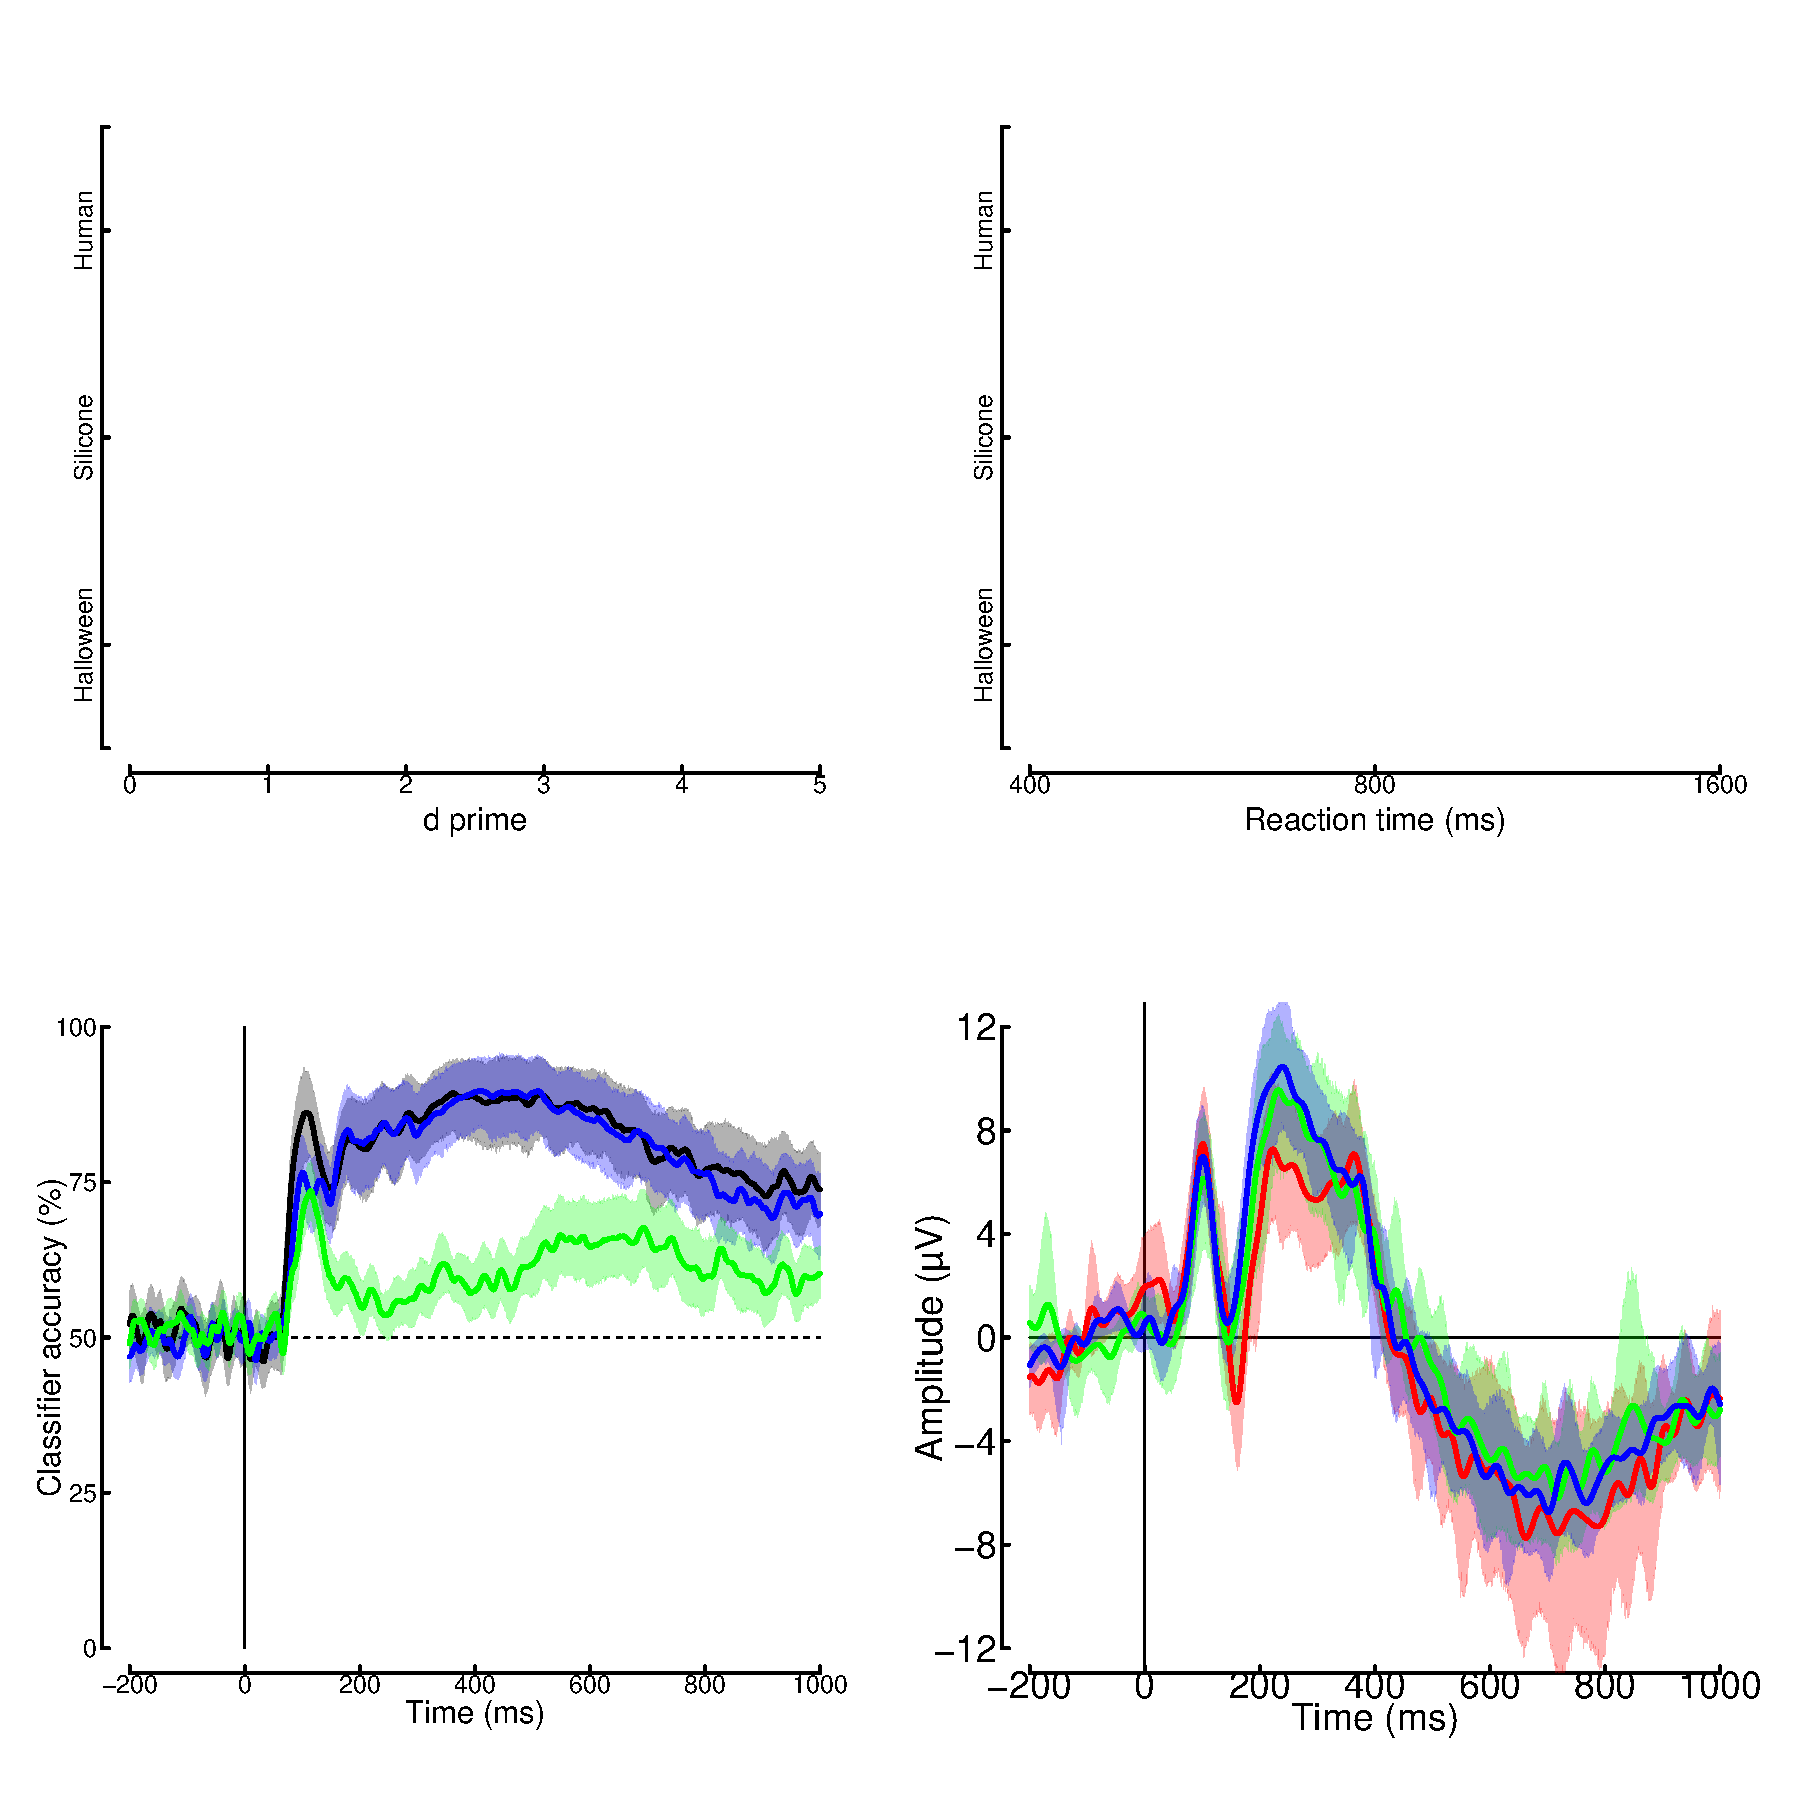
\includegraphics{Figures/MaskData} 

}

\caption{I.}\label{fig:MasksData}
\end{figure}

\begin{figure}

{\centering 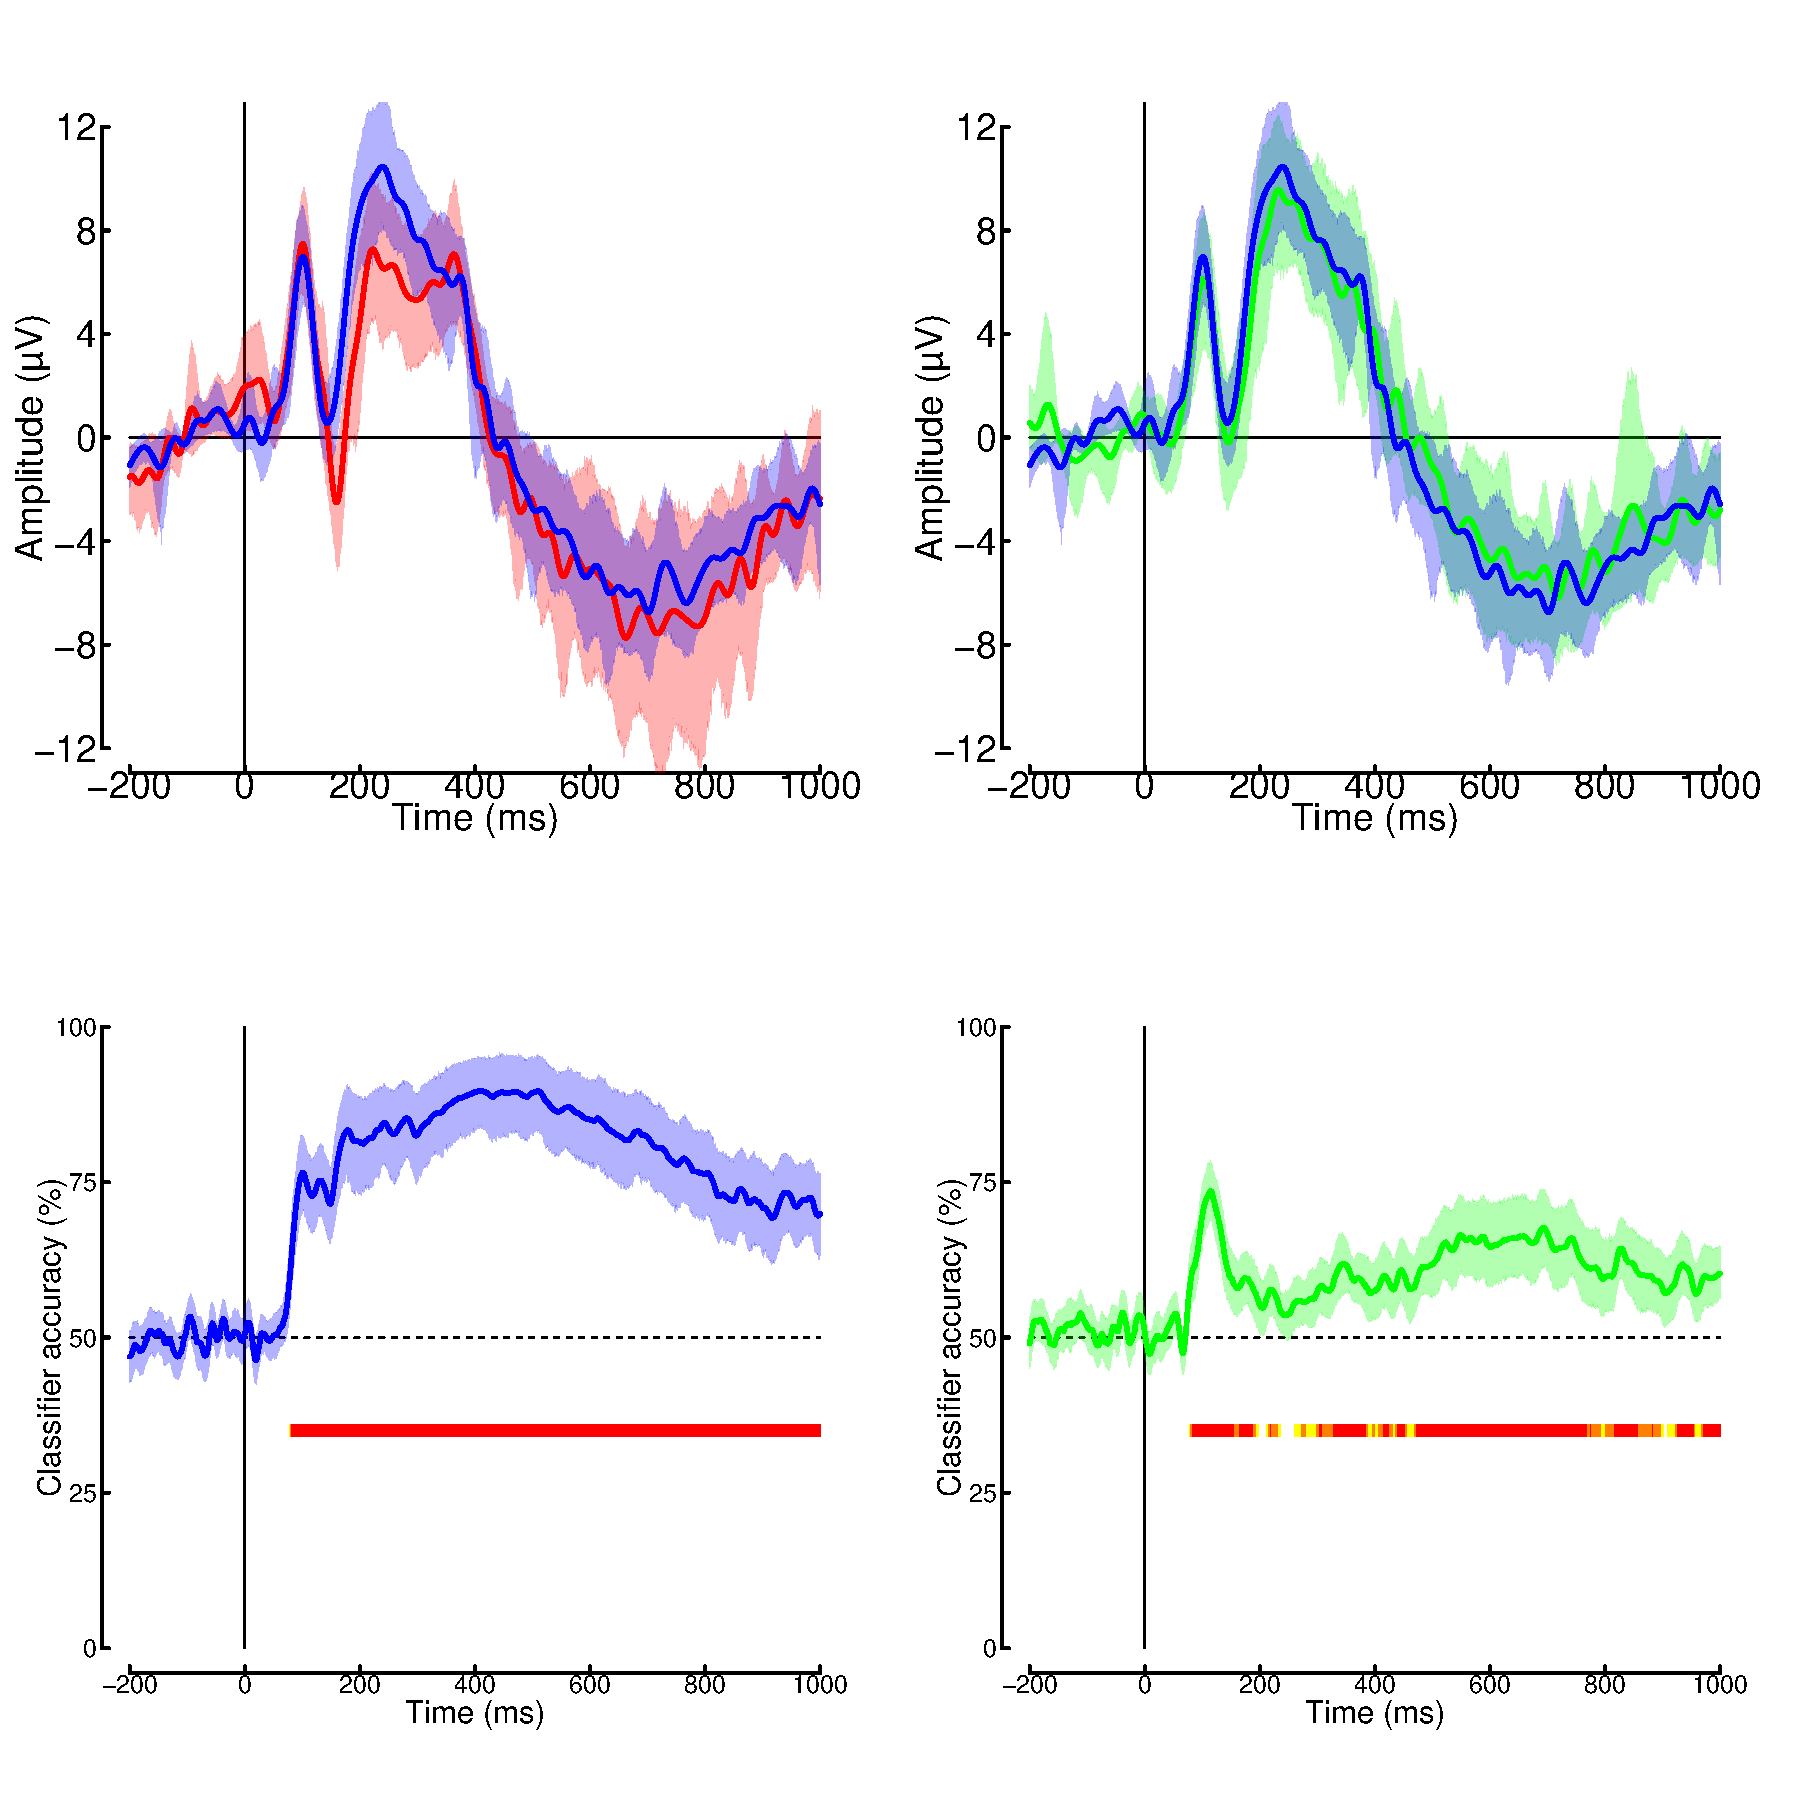
\includegraphics{Figures/MaskMVPA} 

}

\caption{I.}\label{fig:MasksMVPA}
\end{figure}

\hypertarget{discussion}{%
\section{Discussion}\label{discussion}}

\hypertarget{conclusions}{%
\section{Conclusions}\label{conclusions}}

\hypertarget{acknowledgements}{%
\section{Acknowledgements}\label{acknowledgements}}

\hypertarget{references}{%
\section*{References}\label{references}}
\addcontentsline{toc}{section}{References}

\hypertarget{refs}{}
\begin{CSLReferences}{1}{0}
\leavevmode\vadjust pre{\hypertarget{ref-Delorme2004}{}}%
Delorme A, Makeig S. 2004. {EEGLAB}: An open source toolbox for analysis of single-trial {EEG} dynamics including independent component analysis. \emph{J Neurosci Methods} \textbf{134}:9--21. doi:\href{https://doi.org/10.1016/j.jneumeth.2003.10.009}{10.1016/j.jneumeth.2003.10.009}

\leavevmode\vadjust pre{\hypertarget{ref-Downing2001}{}}%
Downing PE, Jiang Y, Shuman M, Kanwisher N. 2001. A cortical area selective for visual processing of the human body. \emph{Science} \textbf{293}:2470--3. doi:\href{https://doi.org/10.1126/science.1063414}{10.1126/science.1063414}

\leavevmode\vadjust pre{\hypertarget{ref-Gauthier2000}{}}%
Gauthier I, Tarr MJ, Moylan J, Skudlarski P, Gore JC, Anderson AW. 2000. The fusiform "face area" is part of a network that processes faces at the individual level. \emph{J Cogn Neurosci} \textbf{12}:495--504. doi:\href{https://doi.org/10.1162/089892900562165}{10.1162/089892900562165}

\leavevmode\vadjust pre{\hypertarget{ref-Hu2020}{}}%
Hu Y, Baragchizadeh A, O'Toole AJ. 2020. Integrating faces and bodies: Psychological and neural perspectives on whole person perception. \emph{Neurosci Biobehav Rev} \textbf{112}:472--486. doi:\href{https://doi.org/10.1016/j.neubiorev.2020.02.021}{10.1016/j.neubiorev.2020.02.021}

\leavevmode\vadjust pre{\hypertarget{ref-Jeffreys1961}{}}%
Jeffreys H. 1961. Theory of probability, 3rd ed. Oxford University Press, Clarendon Press.

\leavevmode\vadjust pre{\hypertarget{ref-Kanwisher1997}{}}%
Kanwisher N, McDermott J, Chun MM. 1997. The fusiform face area: A module in human extrastriate cortex specialized for face perception. \emph{J Neurosci} \textbf{17}:4302--11. doi:\href{https://doi.org/10.1523/JNEUROSCI.17-11-04302.1997}{10.1523/JNEUROSCI.17-11-04302.1997}

\leavevmode\vadjust pre{\hypertarget{ref-Mori1970}{}}%
Mori M. 1970. The uncanny valley. \emph{Energy} \textbf{7}:33--35.

\leavevmode\vadjust pre{\hypertarget{ref-Mori2012}{}}%
Mori M, MacDorman KF, Kageki N. 2012. The uncanny valley {[}from the field{]}. \emph{IEEE Robotics \& Automation Magazine} \textbf{19}:98--100. doi:\href{https://doi.org/10.1109/MRA.2012.2192811}{10.1109/MRA.2012.2192811}

\leavevmode\vadjust pre{\hypertarget{ref-Rouder2009}{}}%
Rouder JN, Speckman PL, Sun D, Morey RD, Iverson G. 2009. Bayesian t tests for accepting and rejecting the null hypothesis. \emph{Psychon Bull Rev} \textbf{16}:225--37. doi:\href{https://doi.org/10.3758/PBR.16.2.225}{10.3758/PBR.16.2.225}

\leavevmode\vadjust pre{\hypertarget{ref-Sanders2017}{}}%
Sanders JG, Ueda Y, Minemoto K, Noyes E, Yoshikawa S, Jenkins R. 2017. Hyper-realistic face masks: A new challenge in person identification. \emph{Cognitive Research: Principles and Implications} \textbf{2}. doi:\href{https://doi.org/10.1186/s41235-017-0079-y}{10.1186/s41235-017-0079-y}

\leavevmode\vadjust pre{\hypertarget{ref-Saygin2012}{}}%
Saygin AP, Chaminade T, Ishiguro H, Driver J, Frith C. 2012. The thing that should not be: Predictive coding and the uncanny valley in perceiving human and humanoid robot actions. \emph{Soc Cogn Affect Neurosci} \textbf{7}:413--22. doi:\href{https://doi.org/10.1093/scan/nsr025}{10.1093/scan/nsr025}

\leavevmode\vadjust pre{\hypertarget{ref-Thierry2007}{}}%
Thierry G, Martin CD, Downing P, Pegna AJ. 2007. Controlling for interstimulus perceptual variance abolishes N170 face selectivity. \emph{Nat Neurosci} \textbf{10}:505--11. doi:\href{https://doi.org/10.1038/nn1864}{10.1038/nn1864}

\leavevmode\vadjust pre{\hypertarget{ref-Urgen2018}{}}%
Urgen BA, Kutas M, Saygin AP. 2018. Uncanny valley as a window into predictive processing in the social brain. \emph{Neuropsychologia} \textbf{114}:181--185. doi:\href{https://doi.org/10.1016/j.neuropsychologia.2018.04.027}{10.1016/j.neuropsychologia.2018.04.027}

\end{CSLReferences}

\end{document}
